\begin{prob}
    Two containers $A$ and $B$ have capacities of 3 liters and 5 liters,
    respectively. Describe how you can measure exactly one liter of water
    using only these two containers. You may 1) fill each container to the
    top using a faucet; 2) completely empty either container into a drain;
    and 3) pour one container into the other until it is empty or the other
    container is full. Both containers are empty to start.

    \begin{responsebox}{6.5in}
        \newcommand{\state}[2]{$\frac{#1}{3}\quad\frac{#2}{5}$}

        \tikzset{
            done/.style={fill=black!10}
        }

        While this may not seem like it, we can think of this as a graph
        problem. Starting with both containers empty, there are two things
        we can do: we can fill container $A$ or fill container $B$. We can depict this situation as follows:
        \begin{center}
            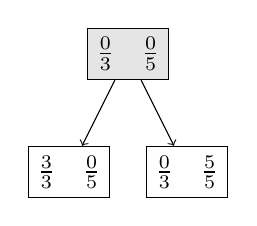
\begin{tikzpicture}[
                    every node/.style={draw},
                    ->
                    ]
                \node[done] {\state{0}{0}}
                    child { node {\state{3}{0}} }
                    child { node {\state{0}{5}} }
                    ;
            \end{tikzpicture}
        \end{center}
        In other words, going from the situation where both containers are
        empty, we can go to either of two new situations: that in which
        container $A$ is full and $B$ is empty, or that where $A$ is empty
        and $B$ is full. In other words, we have a graph in which each node
        represents a state of the world, and we have an edge between two
        nodes if we can get from one state to the other. We are in search
        of a node where one of the containers contains exactly 1 liter.

        We have colored the starting node gray in the above depiction to
        denote that we have already enumerated all of the situations that
        can be reached in one step, starting at that node. The other nodes
        are still uncolored: we need to enumerate their successors.

        Our next step is to further expand the graph. Suppose we are at the
        left node in which $A$ is full and $B$ is empty. There are 
        \begin{enumerate}
            \item Pour out $A$. This takes us back to the starting node in
                which both containers are empty. We could draw an edge back
                to it, but let's not, since returning to the start cannot
                get us closer to the solution, and drawing the edge will
                only clutter the picture.
            \item Pour $A$ into $B$. This results in $A$ being empty and
                $B$ having 3 liters.
            \item Fill $B$ from the faucet. This
                results in $A$ having 3 liters and $B$ having 5.
        \end{enumerate}
        We can depict these steps with the following graph:
        \begin{center}
            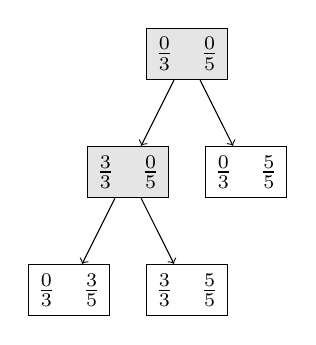
\begin{tikzpicture}[
                    every node/.style={draw},
                    ->
                    ]
                \node[done] {\state{0}{0}}
                    child { node[done] {\state{3}{0}} 
                        child { node {\state{0}{3} } }
                        child { node (x) {\state{3}{5} } }
                    }
                    child { node {\state{0}{5}} }
                    ;
            \end{tikzpicture}
        \end{center}
        We still haven't found a solution node yet. Let's expand the \tikz{\node[draw]{\state{0}{5}}} node.
        There are several things we can do:
        \begin{enumerate}
            \item Pour out $B$. This takes us back to the starting node in
                which both containers are empty. We could draw an edge back
                to it, but we won't for the same reasons given above.
            \item Pour $B$ into $A$ until $A$ is full. This results in $A$
                having 3 liters and $B$ having 2 liters.
            \item Fill $A$ from the faucet. This results in $A$ having 3
                liters and $B$ having 5. We already have such a node, and
                we could draw an edge to it, but we won't for the reasons
                given above.
        \end{enumerate}
        Our graph becomes:
        \begin{center}
            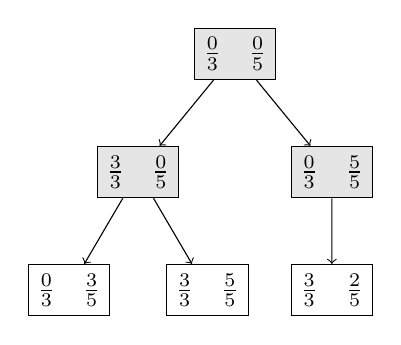
\begin{tikzpicture}[
                    every node/.style={draw},
                    ->,
                    level 1/.style={sibling distance=7em},
                    level 2/.style={sibling distance=5em}
                    ]
                \node[done] {\state{0}{0}}
                    child { node[done] {\state{3}{0}} 
                        child { node {\state{0}{3} } }
                        child { node (x) {\state{3}{5} } }
                    }
                    child { node[done] {\state{0}{5}} 
                        child { node {\state{3}{2}}  }
                    }
                    ;
            \end{tikzpicture}
        \end{center}
        Continuing this process for several more steps, we will arrive at:
        \begin{center}
            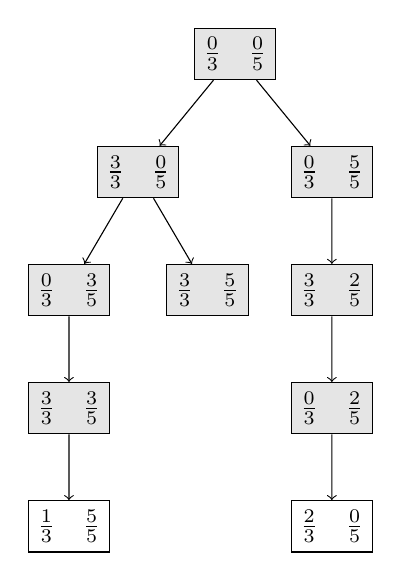
\begin{tikzpicture}[
                    every node/.style={draw},
                    ->,
                    level 1/.style={sibling distance=7em},
                    level 2/.style={sibling distance=5em}
                    ]
                \node[done] {\state{0}{0}}
                    child { node[done] {\state{3}{0}} 
                        child { node[done] {\state{0}{3} } 
                            child { node[done] {\state{3}{3} } 
                                child { node {\state{1}{5}} }
                            }
                        }
                        child { node[done] (x) {\state{3}{5} } }
                    }
                    child { node[done] {\state{0}{5}} 
                        child { node[done] {\state{3}{2}}
                            child { node[done] {\state{0}{2}} 
                                child { node {\state{2}{0}} }
                            }
                        }
                    }
                    ;
            \end{tikzpicture}
        \end{center}
        We have found a node in which container $A$ contains 1 liter. We can
        describe the process followed by taking the path from the root node
        to this node:
        \begin{enumerate}
            \item Fill $A$ from the faucet: \state30
            \item Pour $A$ into $B$: \state03
            \item Fill $A$ from the faucet: \state33
            \item Pour $A$ into $B$: \state15
        \end{enumerate}


    \end{responsebox}
\end{prob}
